\documentclass{anstrans}
%%%%%%%%%%%%%%%%%%%%%%%%%%%%%%%%%%%
\title{Validation of Spent Nuclear Fuel Output by Cyclus, a Fuel Cycle Simulator Code}
\author{Gwendolyn J. Chee, Gyutae Park, and Kathryn D. Huff}

\institute{
Dept. of Nuclear, Plasma and Radiological Engineering, University of Illinois at Urbana-Champaign \\
gchee2@illinois.edu
}

%%%% packages and definitions (optional)
\usepackage{graphicx} % allows inclusion of graphics
\usepackage{booktabs} % nice rules (thick lines) for tables
\usepackage{microtype} % improves typography for PDF
\usepackage{xspace}
\usepackage{tabularx}
\usepackage{subcaption}
\newcommand{\SN}{S$_N$}
\renewcommand{\vec}[1]{\bm{#1}} %vector is bold italic
\newcommand{\vd}{\bm{\cdot}} % slightly bold vector dot
\newcommand{\grad}{\vec{\nabla}} % gradient
\newcommand{\ud}{\mathop{}\!\mathrm{d}} % upright derivative symbol
\newcommand{\Cyclus}{\textsc{Cyclus}\xspace}%
\newcommand{\Cycamore}{\textsc{Cycamore}\xspace}%
\newcolumntype{c}{>{\hsize=.56\hsize}X}
\newcolumntype{b}{>{\hsize=.7\hsize}X}
\newcolumntype{s}{>{\hsize=.74\hsize}X}
\newcolumntype{f}{>{\hsize=.1\hsize}X}
\newcolumntype{a}{>{\hsize=.45\hsize}X}
\usepackage{titlesec}
\titleformat*{\subsection}{\normalfont}

\begin{document}
%%%%%%%%%%%%%%%%%%%%%%%%%%%%%%%%%%%%%%%%%%%%%%%%%%%%%%%%%%%%%%%%%%%%%%%%%%%%%%%%
\section{Introduction}
\Cyclus \cite{carlsen_cyclus_2014} , a fuel cycle simulator, was used to simulate the
United States' nuclear fuel cycle from 1967 up till 2013. The \Cyclus spent nuclear fuel (SNF) data was compared to SNF data from the U.S Department of Energy (DOE) sponsored Unified Database (UDB) \cite{peterson_unf-st&dards_2017}. The UDB provides comprehensive and consistent technical data on reactor sites and spent nuclear fuel (SNF) from the beginning of nuclear reactor operation in the United States till 2013. Comparison of both sets of data establishes baseline comparison models between \Cyclus simulated results and real world metrics. 

%%% 
\section{Background}
\Cyclus is an agent-based extensible framework for modeling flow of material through user-defined nuclear fuel cycles \cite{huff_fundamental_2016}. \Cycamore \cite{carlsen_cycamore_2014} is an additional modules repository in the \Cyclus ecosystem that provides basic libraries to represent process physics of various components of the nuclear fuel cycle (ie. mining, fuel enrichment, reactor) \cite{huff_extensions_2014}. Each library is an archetype. 

%%%%%%%%%%%%%%%%%%%%%%%%%%%%%%%%%%%%%%%%%%%%%%%%%%%%%%%%%%%%%%%%%%%%%%%%%%%%%%%%
\section{Motivation}
The United States is currently considering various fuel cycles and geologic disposal options
\cite{DOE_strategy_2013}. These decisions made will be influenced by key criteria such as thermal load of waste packages and the thermal capacity of the selected geologic host media. Temperature information of the waste packages depend on the decay heat contribution from spent fuel isotopic composition. Accurate spent fuel isotopic composition data gives accurate thermal load data. Therefore, to accurately simulate thermal loading in \Cyclus, the simulation must first give isotopic composition and spent fuel mass that closely replicates reality. 

%%%%%%%%%%%%%%%%%%%%%%%%%%%%%%%%%%%%%%%%%%%%%%%%%%%%%%%%%%%%%%%%%%%%%%%%%%%%%%%%
\section{Methodology}
\subsection{\textit{Generating \Cyclus Simulation and Analysis}}
A \Cyclus simulation of the United States Nuclear Fuel Cycle was created using published data about the 112 commerical nuclear reactors that have operated since 1967 in the United States. The reactor deployment data was obtained from the Power Reactor Information System's (PRIS) reactor database \cite{IAEA_pris_2017}. The relevant data included: country, reactor unit, type, net capacity (MWe), first grid date and shutdown date. From there, data for reactors in the United States were extracted and used to populate the simulation. The depletion calculations for the nuclear fuel in reactors in the simulation are recipe based, which means that isotopic composition recipes for fresh and spent fuel are used. The recipes are taken from a reference depletion calculation from ORIGEN. The recipe was also used in \cite{wilson_adoption_2009, bae_synergistic_2017}. 

Jinja2 \cite{ronacher_welcome_2018}, a Python templating language, was then used in Python to render the data into an input file that can be accepted by \Cyclus. The output file produced by \Cyclus was also analyzed using Python. 

The assumptions made for this \Cyclus simulation include: 

\begin{enumerate}
	\item Decay is not taken into account. 
	\item Reactors are assumed to have a lifetime of 60 years unless shut down prematurely.
	\item Cycle time is assumed to be 18 months. 
	\item Refuel time is assumed to be 1 month. 
\end{enumerate}


\subsection{\textit{UDB Data Analysis}}
The UDB data contained SNF information from 1967 up to 2013. The dataset includes discharged fuel assembly data per reactor, specific isotopic concentrations and decay heat for each assembly along with its discharge date \cite{peterson_unf-st&dards_2017}. UDB was imported into Python and processed to be compared with \Cyclus simulation output. All scripts and data used are available in \cite{chee_arfc/transition-scenarios_2018}. 
%%%%%%%%%%%%%%%%%%%%%%%%%%%%%%%%%%%%%%%%%%%%%%%%%%%%%%%%%%%%%%%%%%%%%%%%%%%%%%%%
\section{Results and Analysis}
The primary outcome of this validation is to provide comparisons between \Cyclus and UDB for spent fuel mass and major isotopic contributions to the total spent fuel mass. 

\subsection{\textit{Cumulative Total Spent Fuel Mass Comparison}}
Figure \ref{fig:total_original} shows the cumulative spent fuel mass for both \Cyclus and UDB data from 1967 to 2013. The total spent fuel mass produced by \Cyclus is larger than UDB data before the year 2000. The \Cyclus and UDB total spent fuel mass data diverge after 2000, with UDB being larger. The discrepancies can be attributed to rigidity of \Cyclus simulation input with respect to cycle and refuel time. In \Cyclus, the user specifies constant month integer refuel and cycle times for each reactor. In reality, the cycle and refuel times are varied throughout each reactor's lifetime and may not fall in exact month spans. 

\begin{figure}[h] % replace 't' with 'b' to force it to be on the bottom
	\centering
	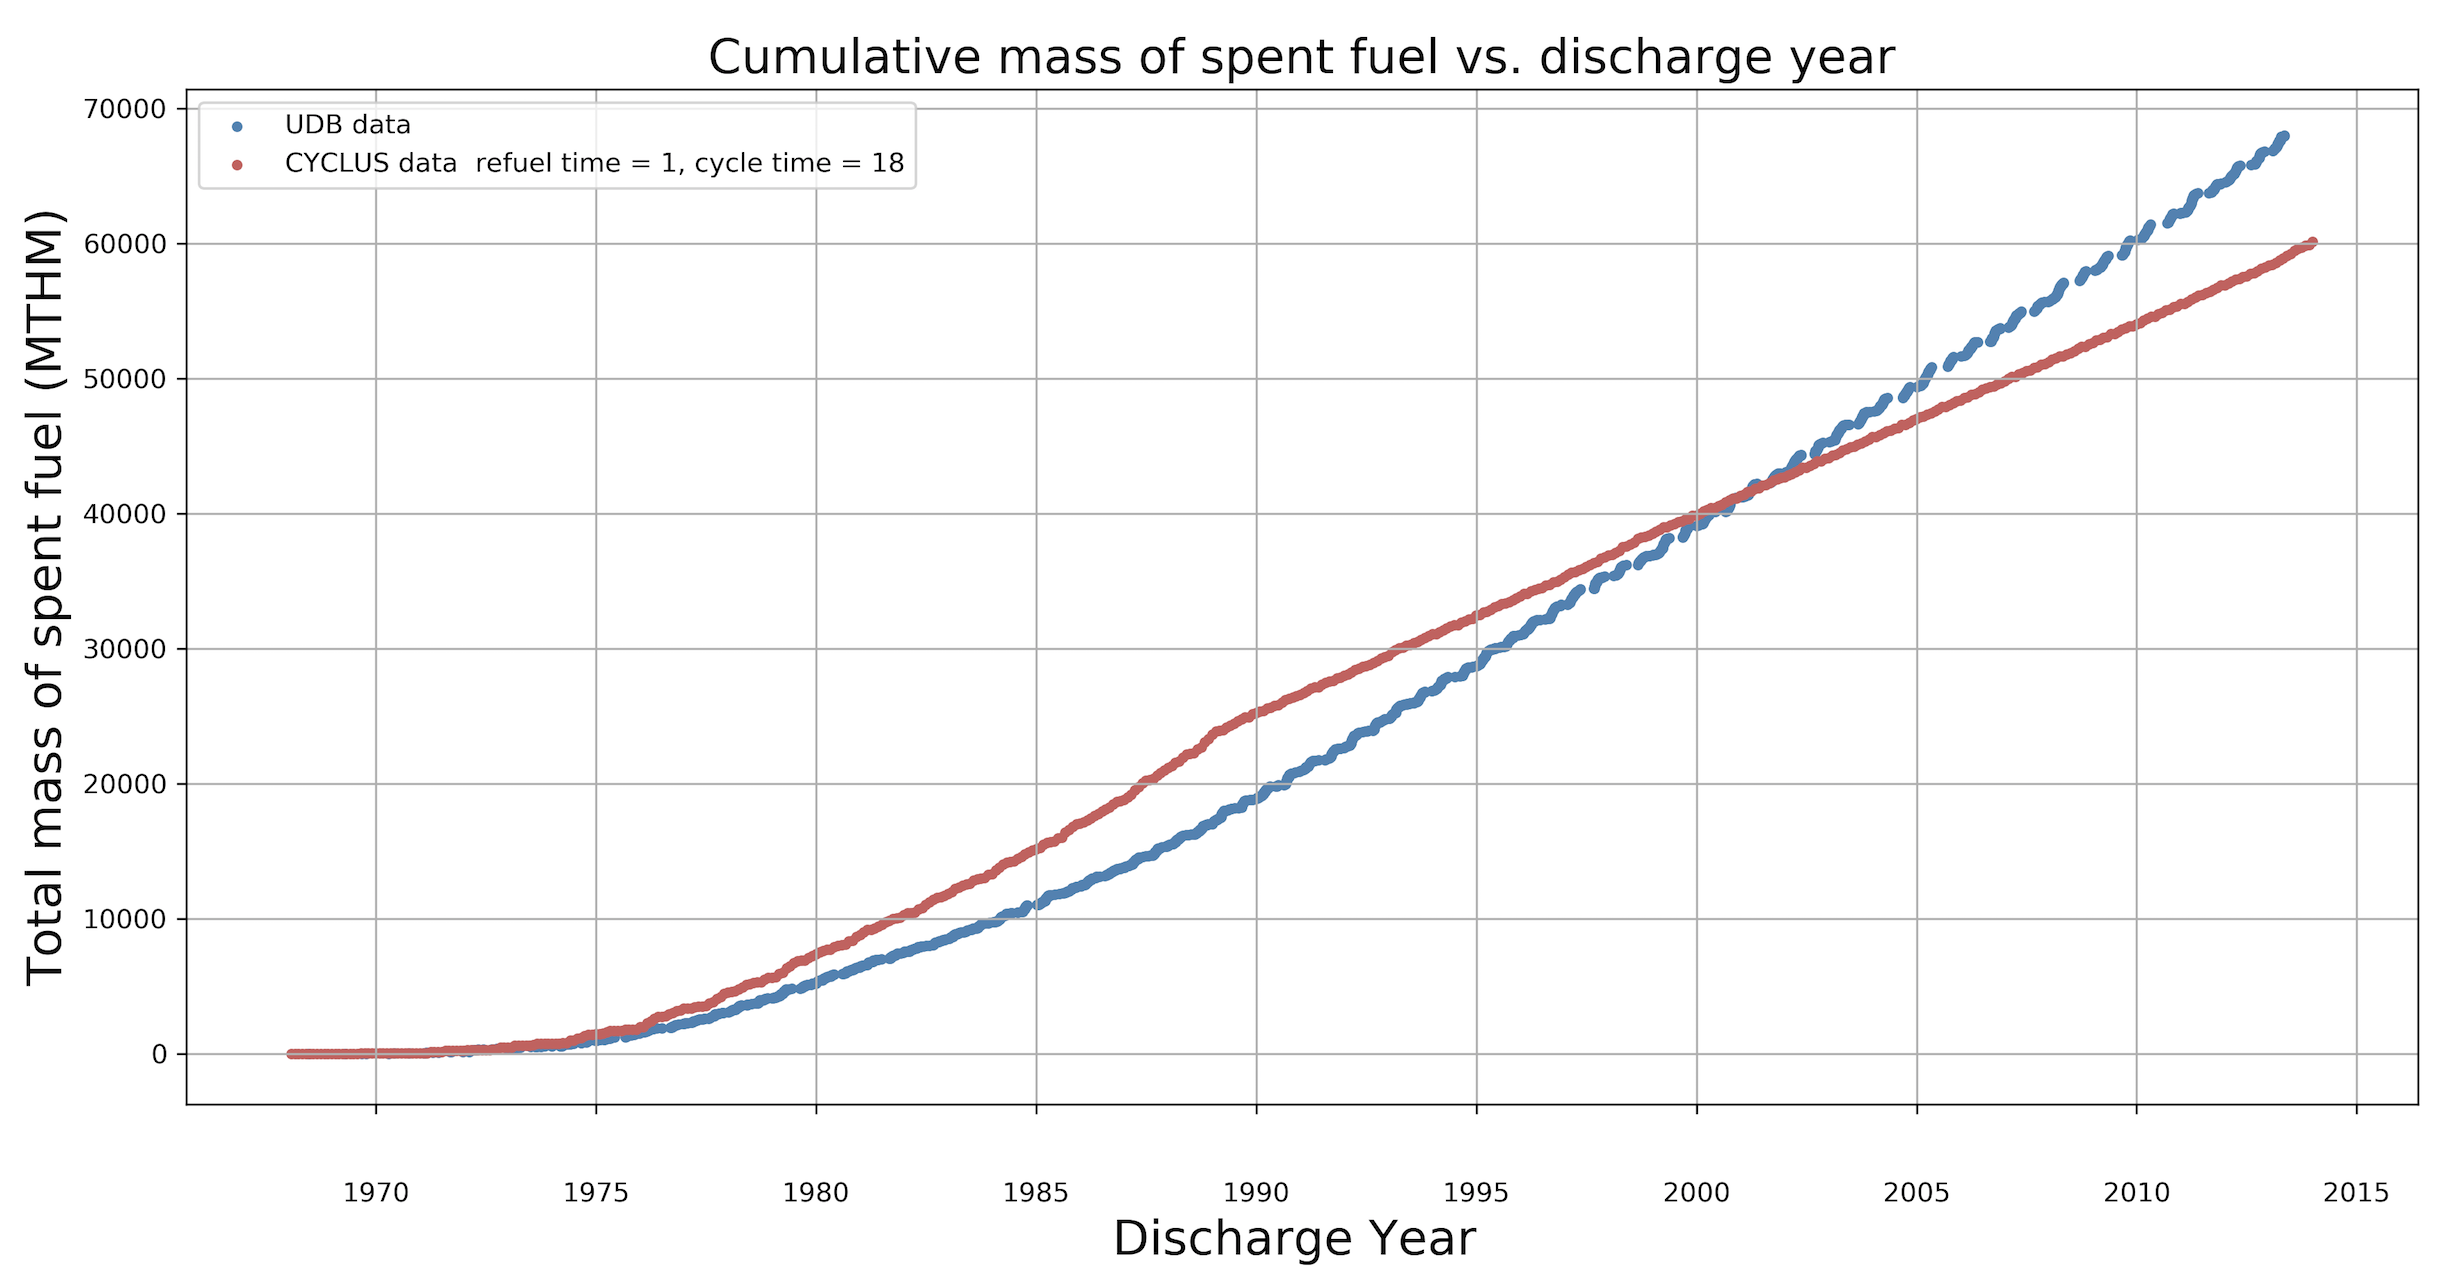
\includegraphics[width=0.48\textwidth]{total_cumulative_mass_spent_fuel_original}
	\caption{Total cumulative spent fuel mass against discharge time for \Cyclus and UDB data from 1967 up to 2013.}
	\label{fig:total_original}
\end{figure}

The Nuclear Energy Institute (NEI) reported that there has been significant variance in the refueling period for reactors in the United States. The average refuelling time in 1990 was 104 days, and generally decreased to an average refuelling time of 35 days in 2017 \cite{iaea_current_nodate}.

\Cyclus' greater spent fuel mass than UDB's before 2000 can be attributed to the assumption that refueling time is always 1 month. Figure \ref{fig:total_refueltime} includes plots of total spent fuel mass from \Cyclus simulations where refuel time is increased. A larger refuel time brings the total spent fuel mass from \Cyclus simulations closer to the UDB data before 2000. 

\begin{figure}[h] 
	\centering
	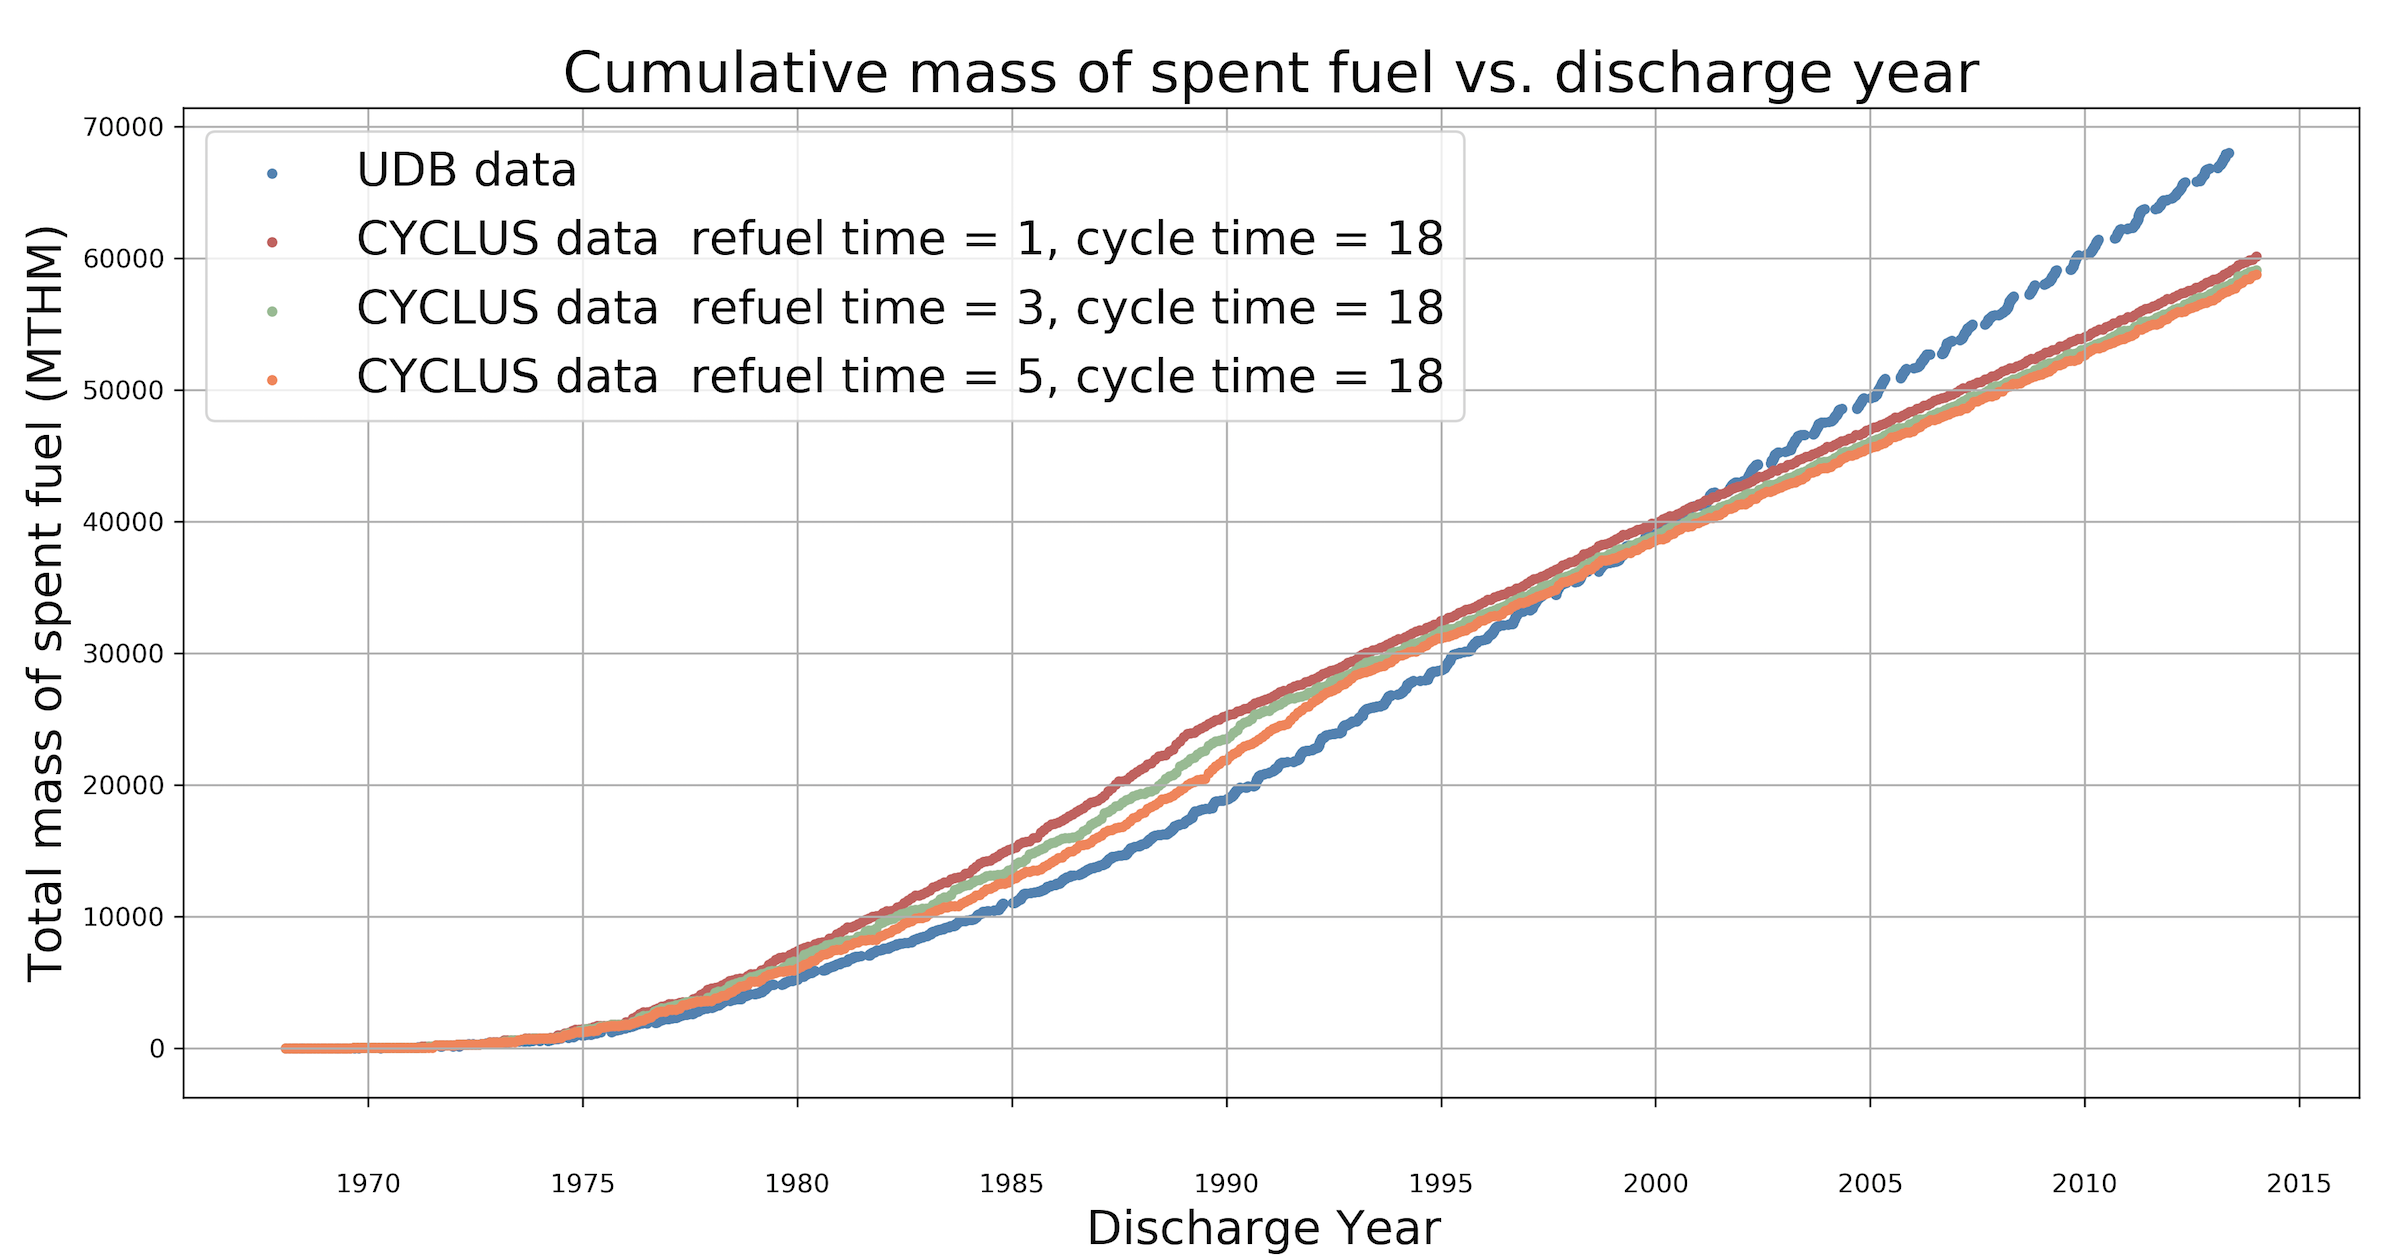
\includegraphics[width=0.48\textwidth]{total_cumulative_mass_spent_fuel_refueltime}
	\caption{Total cumulative spent fuel mass against discharge time for \Cyclus and UDB data from 1967 up to 2013 for varying refuel time}
	\label{fig:total_refueltime}
\end{figure} 

The higher cumulative UDB spent fuel mass compared to \Cyclus' data after 2000 can be attributed to the cycle length of reality being shorter than the 18 month length of \Cyclus simulations. The United States DOE reported that there was a downward trend of forced outage rates of nuclear reactors from 2000 to 2014. The forced outage rate was 4.24\% in 2000 and 2.98\% in 2013 \cite{gehin_nuclear_2016}. As the rate of forced outages decreased from 2000 to 2013, the cycle length also decreases. 

Figure \ref{fig:total_cycletime} includes plots of total spent fuel mass from \Cyclus simulations where cycle time is varied. A shorter cycle time brings the total spent fuel mass from \Cyclus simulations closer to the UDB data after 2000. 

\begin{figure}[h] % replace 't' with 'b' to force it to be on the bottom
	\centering
	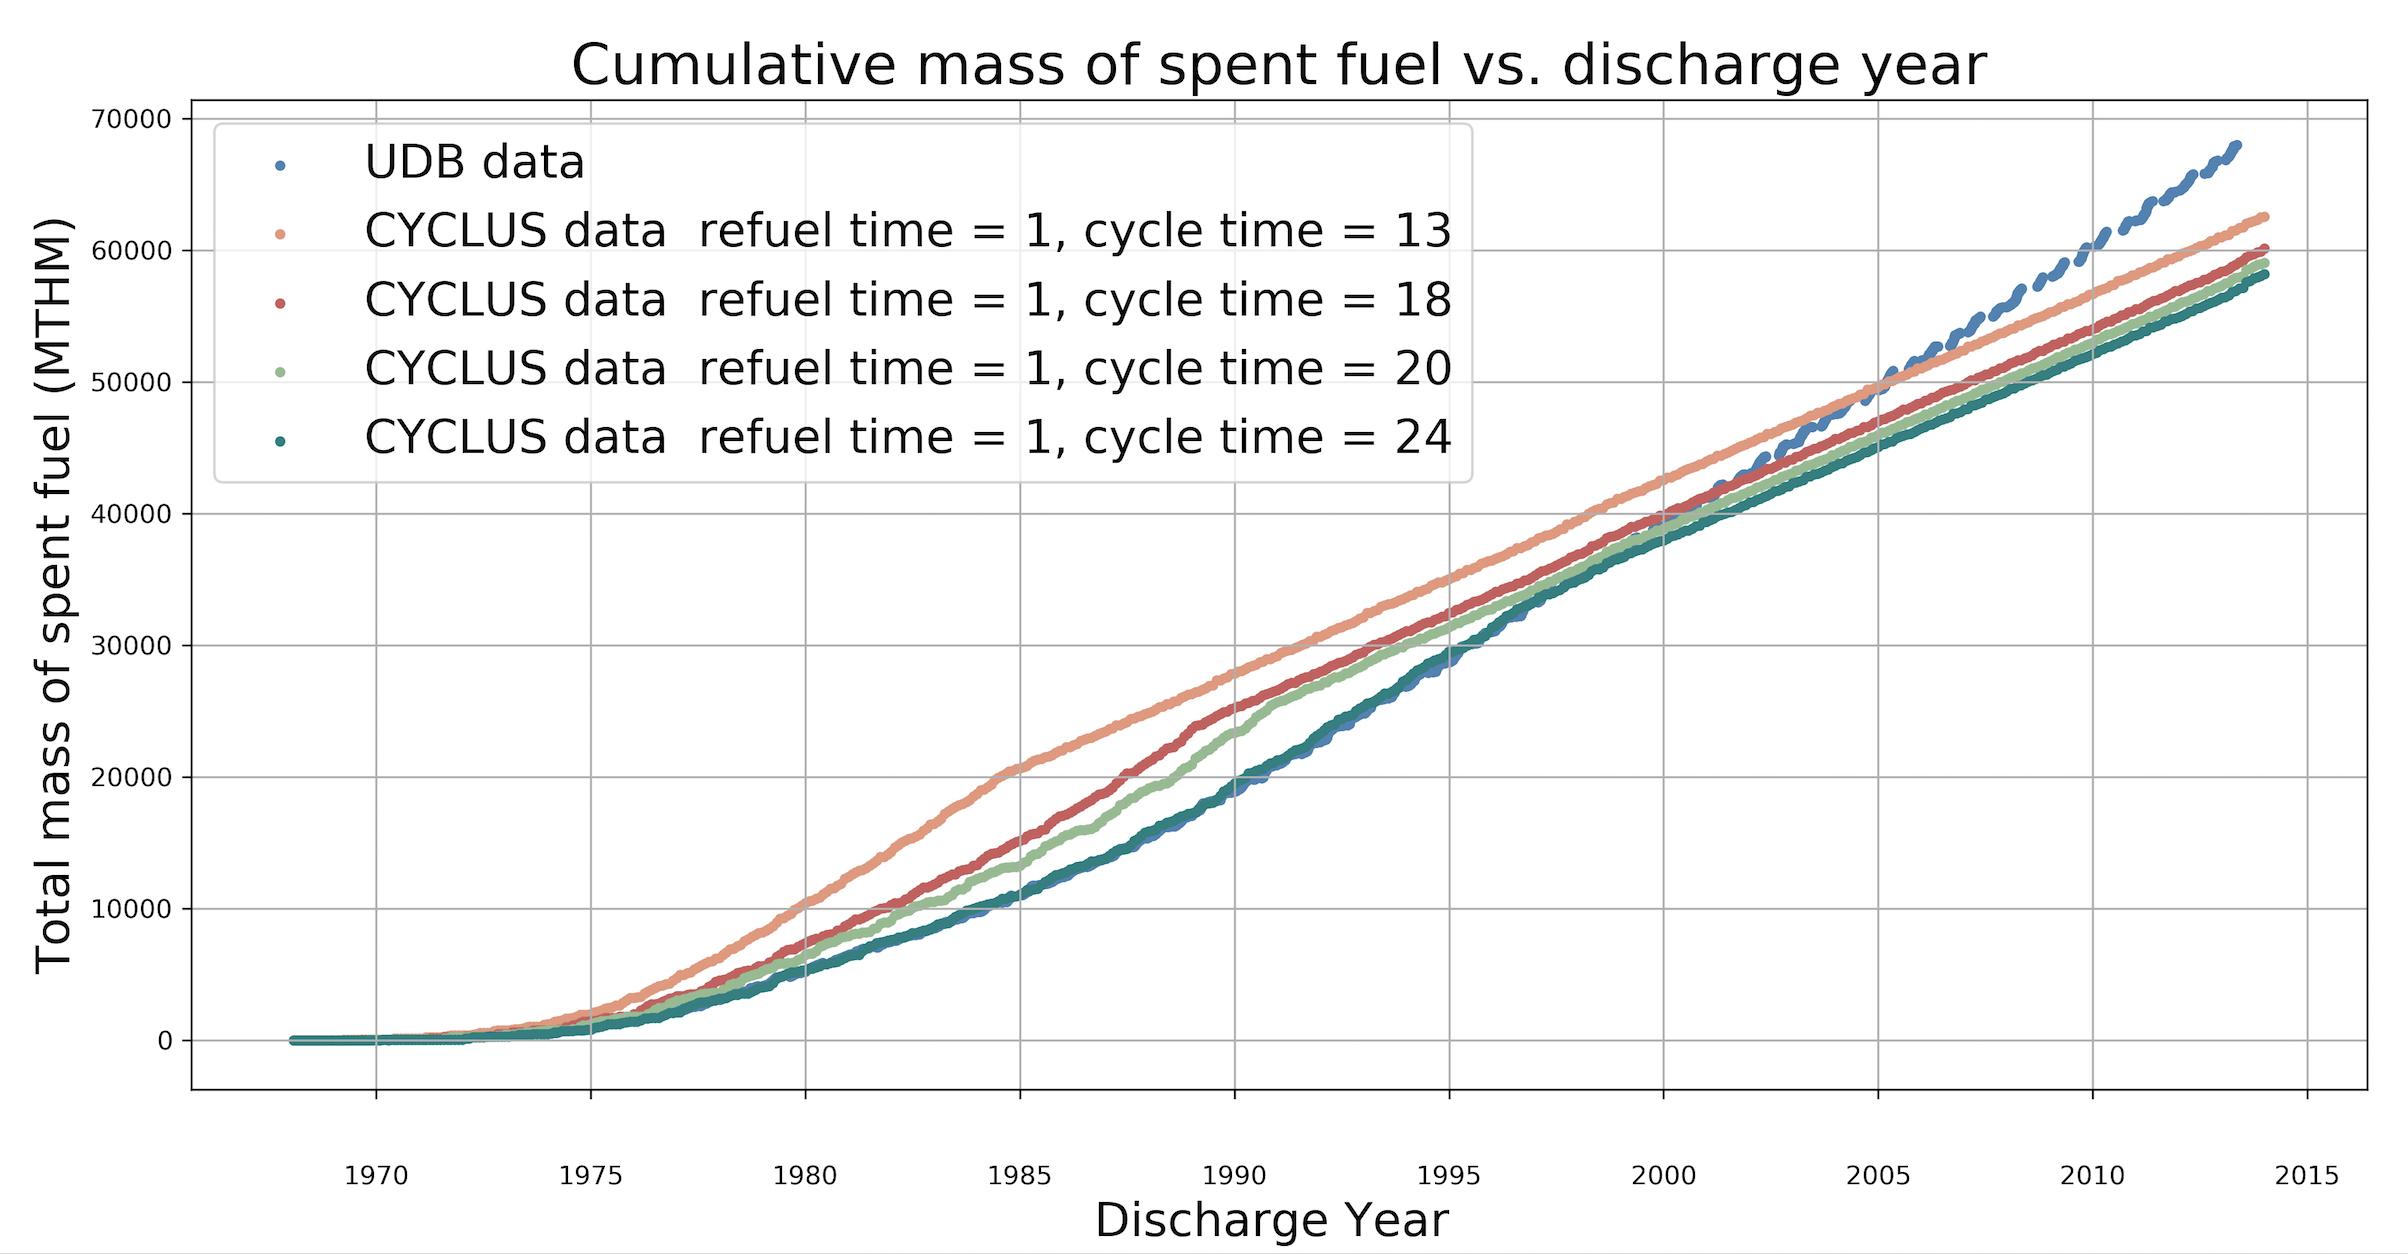
\includegraphics[width=0.48\textwidth]{total_cumulative_mass_spent_fuel_cycletime}
	\caption{Total cumulative spent fuel mass against discharge time for \Cyclus and UDB data from 1967 to 2013 for varying cycle time}
	\label{fig:total_cycletime}
\end{figure} 

\subsection{\textit{Major Isotopic Composition of  Spent Fuel Mass Comparison}}
The three isotopes that contribute the most to the total mass of the spent fuel in order of significance are: U-238, U-235, Pu-239.  

Figure \ref{fig:total_u238}, \ref{fig:total_u235} and \ref{fig:total_pu240} shows the cumulative spent fuel mass for U-238, U-235 and Pu-239 isotope for both \Cyclus and UDB data from 1967 to 2013.
They follow the same trend as figure \ref{fig:total_original} and the same explanations can be used to explain the differences in values. 

\begin{figure}[h]
	\centering
	\begin{subfigure}[b]{0.45\textwidth}
		\centering
		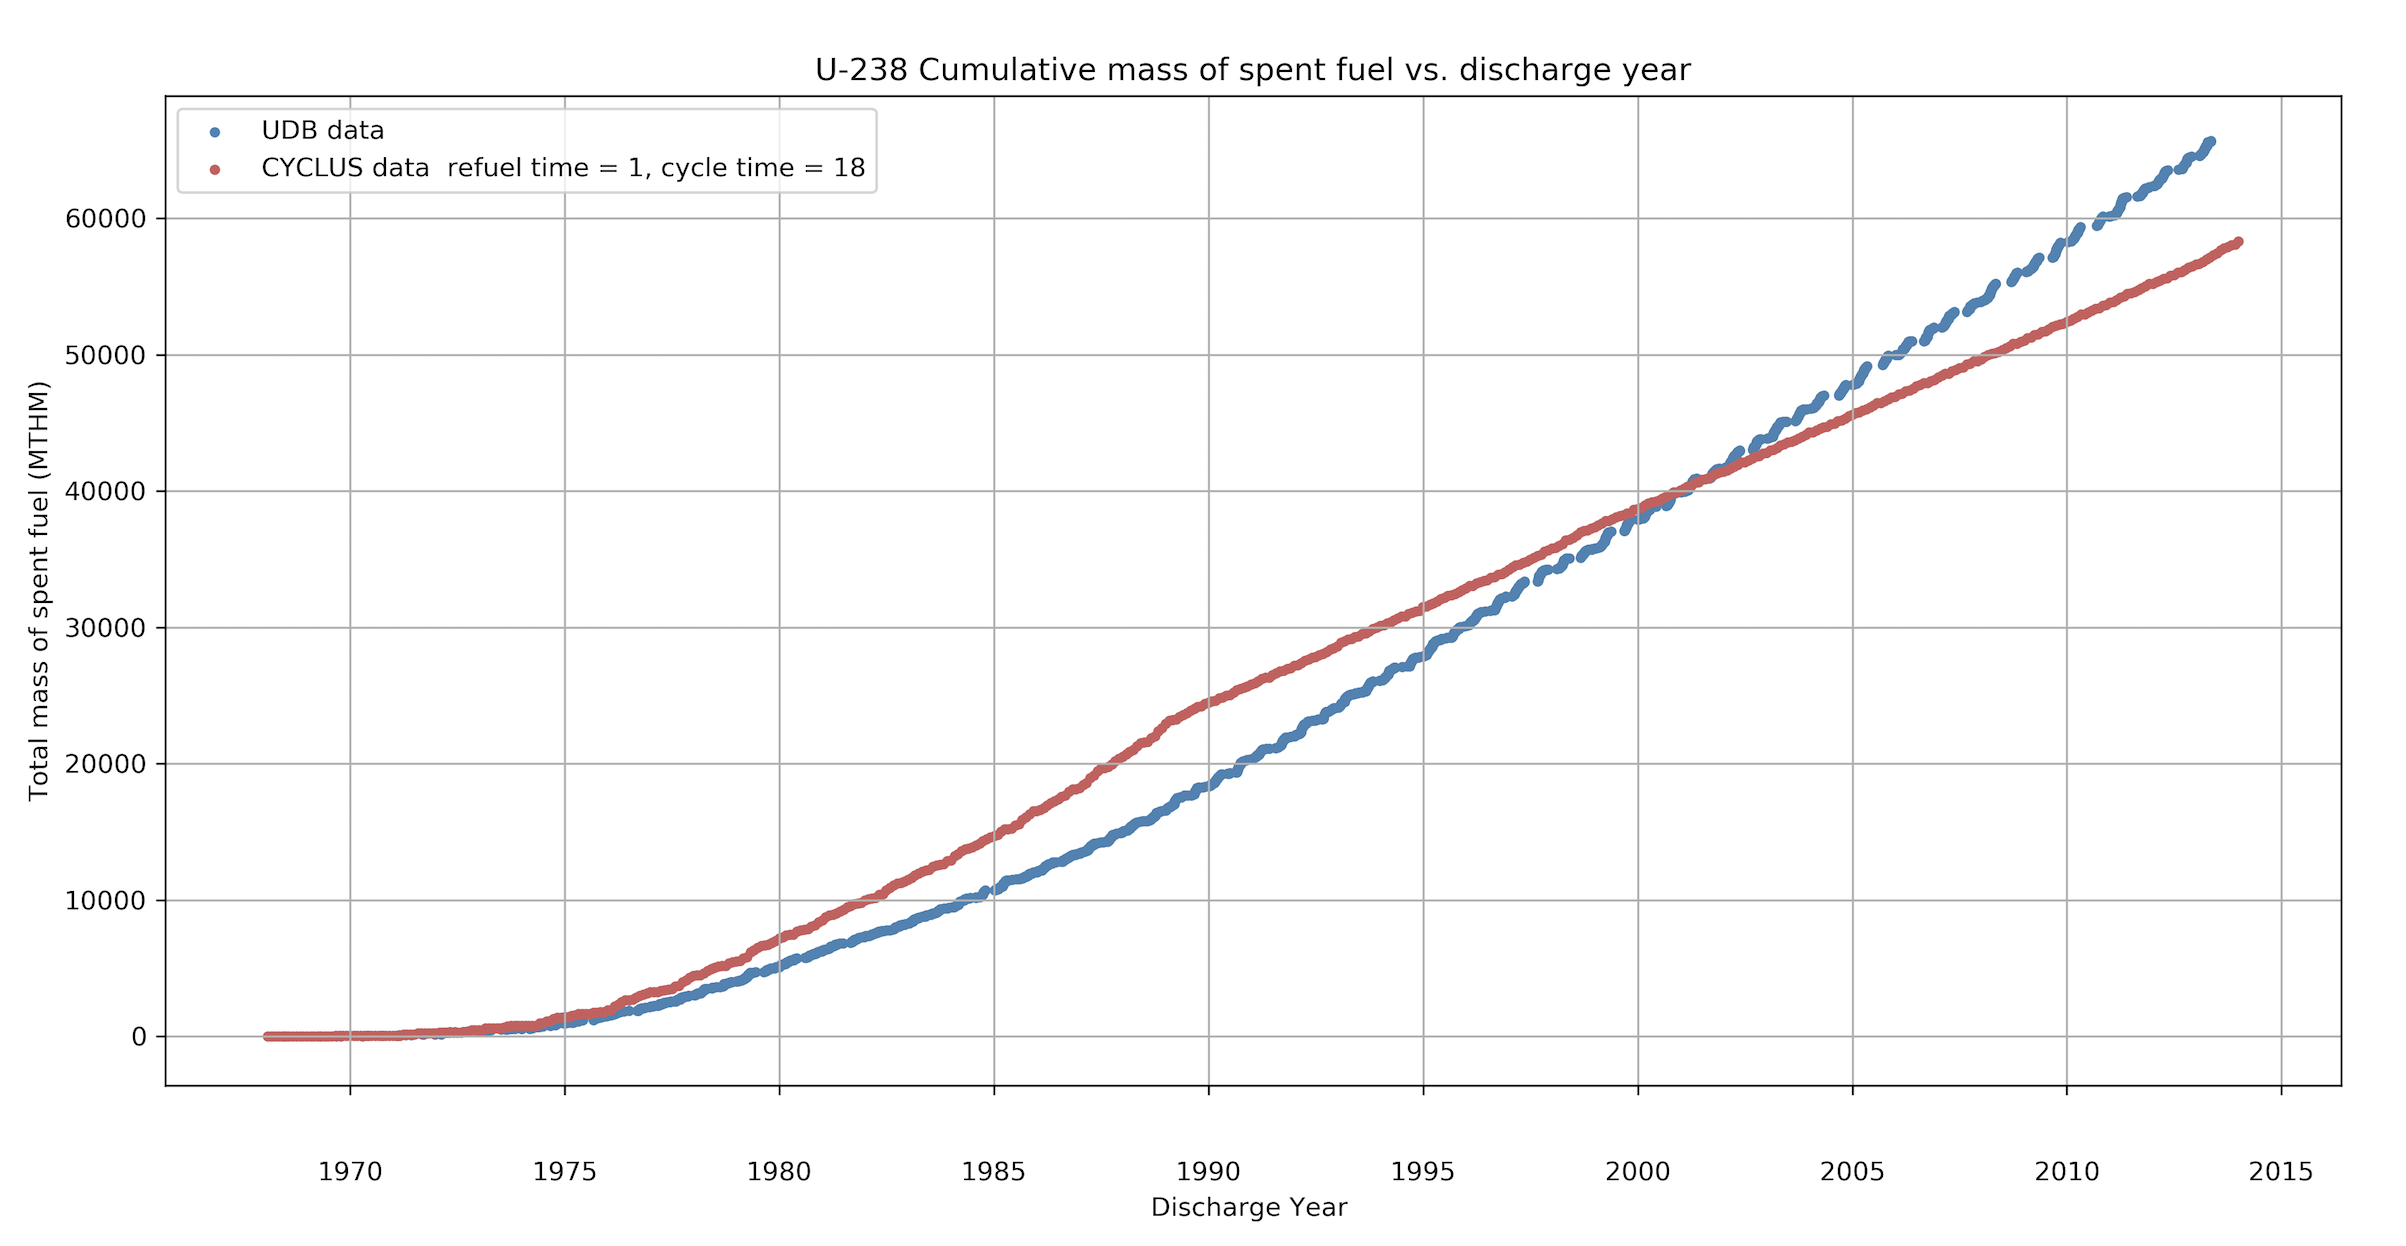
\includegraphics[width=\textwidth]{U-238_cumulative_mass_spent_fuel_original}
		\caption[Network2]%
		{{\small Total cumulative U-238 mass in spent fuel against discharge time for \Cyclus and UDB from 1967 to 2013}}    
		\label{fig:total_u238}
	\end{subfigure}
	\hfill
	\begin{subfigure}[b]{0.45\textwidth}  
		\centering 
		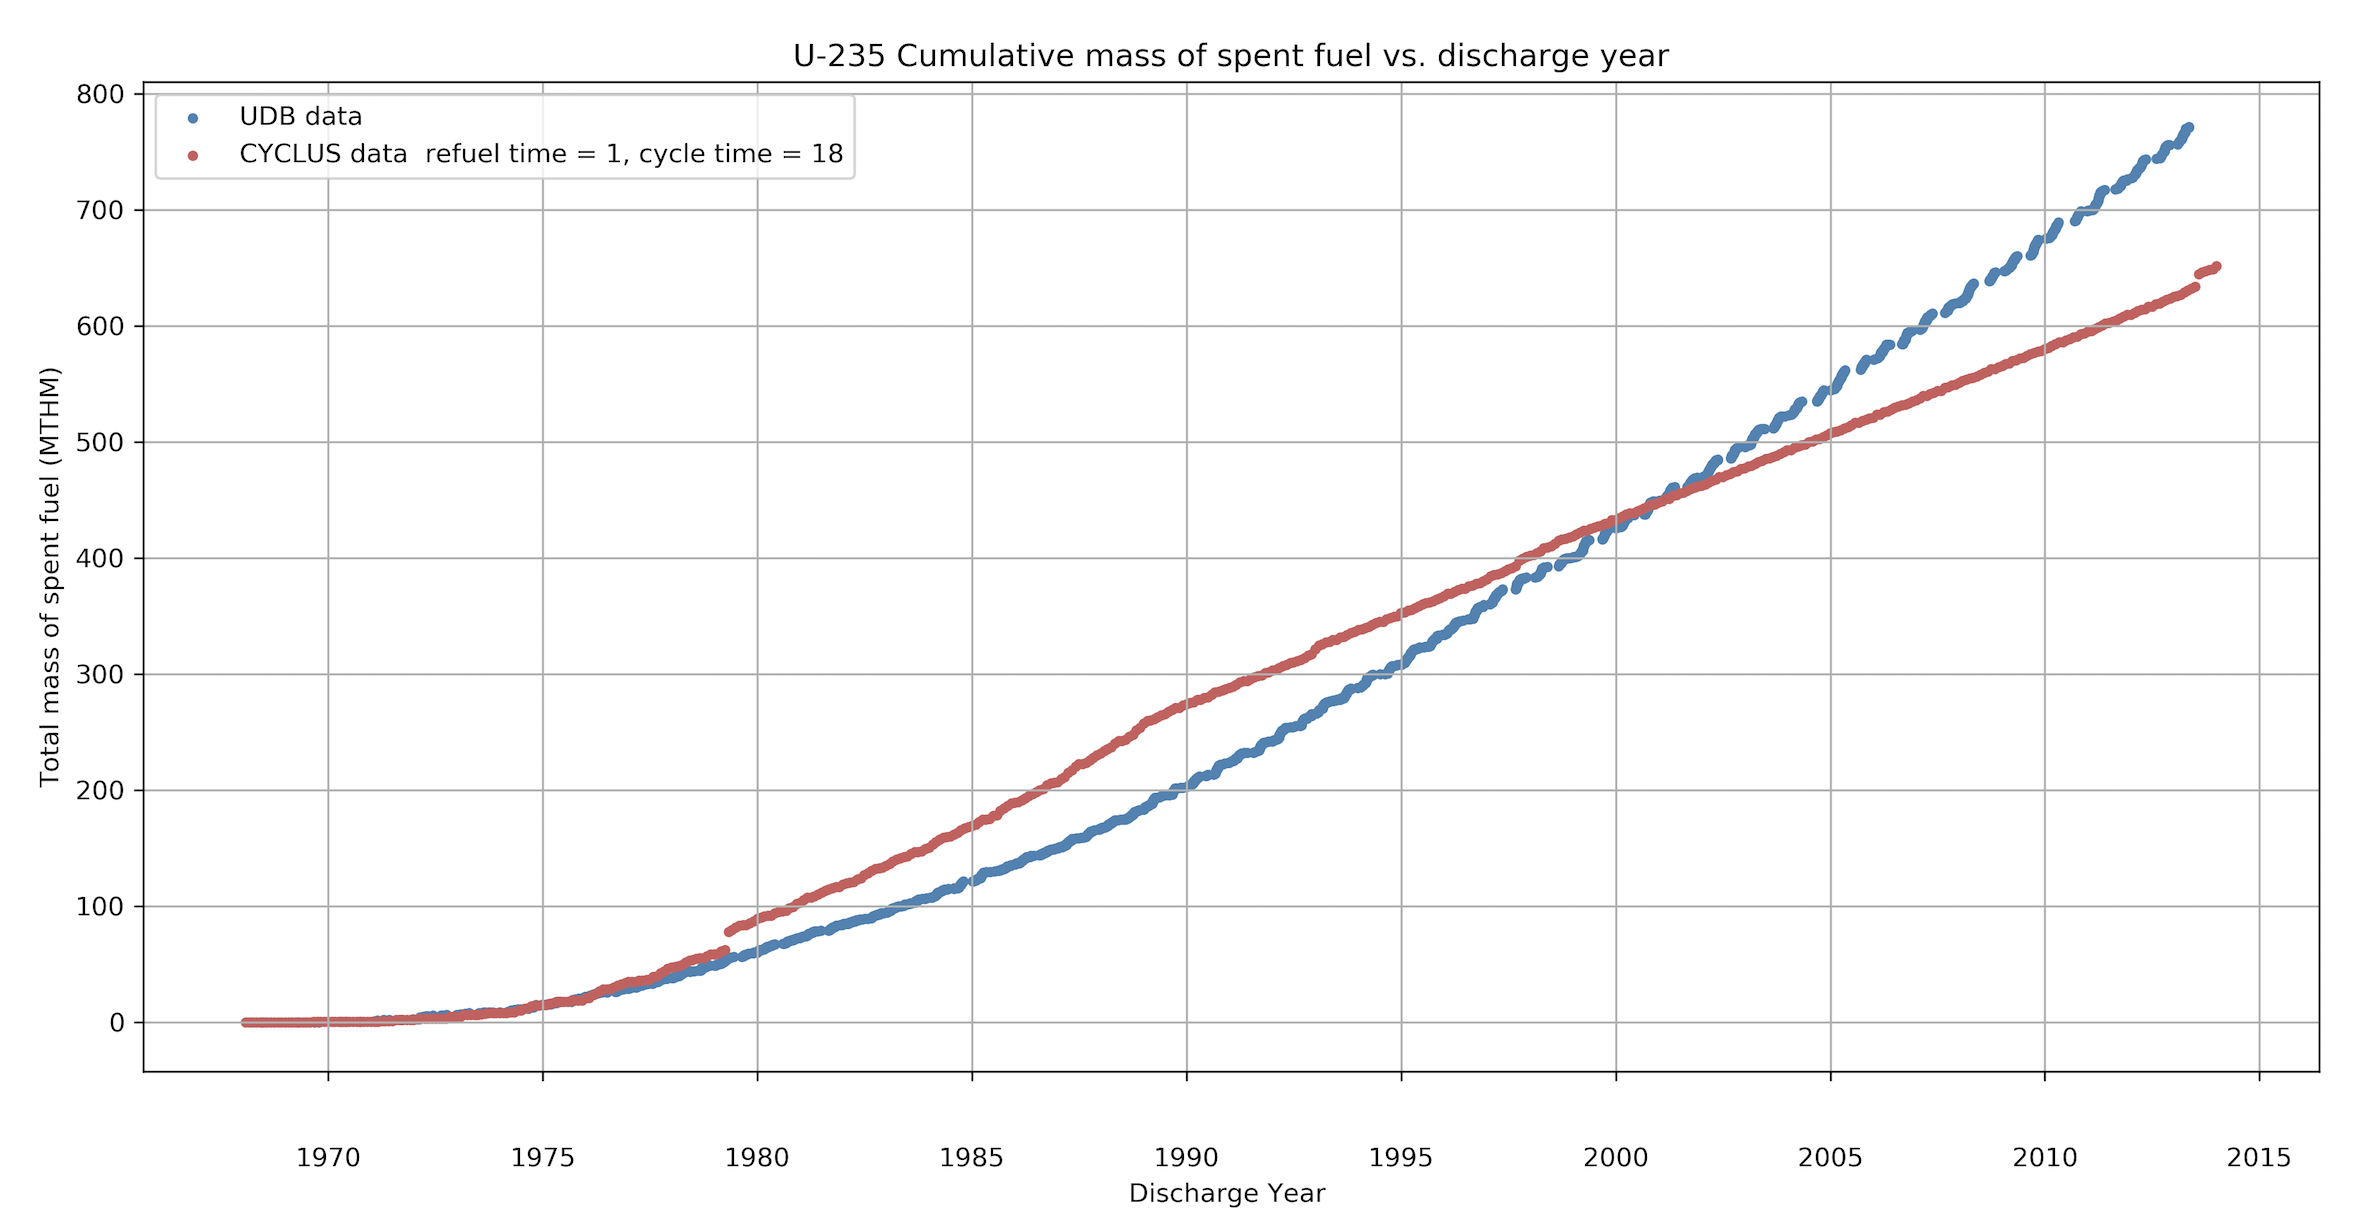
\includegraphics[width=\textwidth]{U-235_cumulative_mass_spent_fuel_original}
		\caption[]%
		{{\small Total cumulative U-235 mass in spent fuel against discharge time for \Cyclus and UDB from 1967 to 2013}}    
		\label{fig:total_u235}
	\end{subfigure}
	\vskip\baselineskip
	\begin{subfigure}[b]{0.45\textwidth}   
		\centering 
		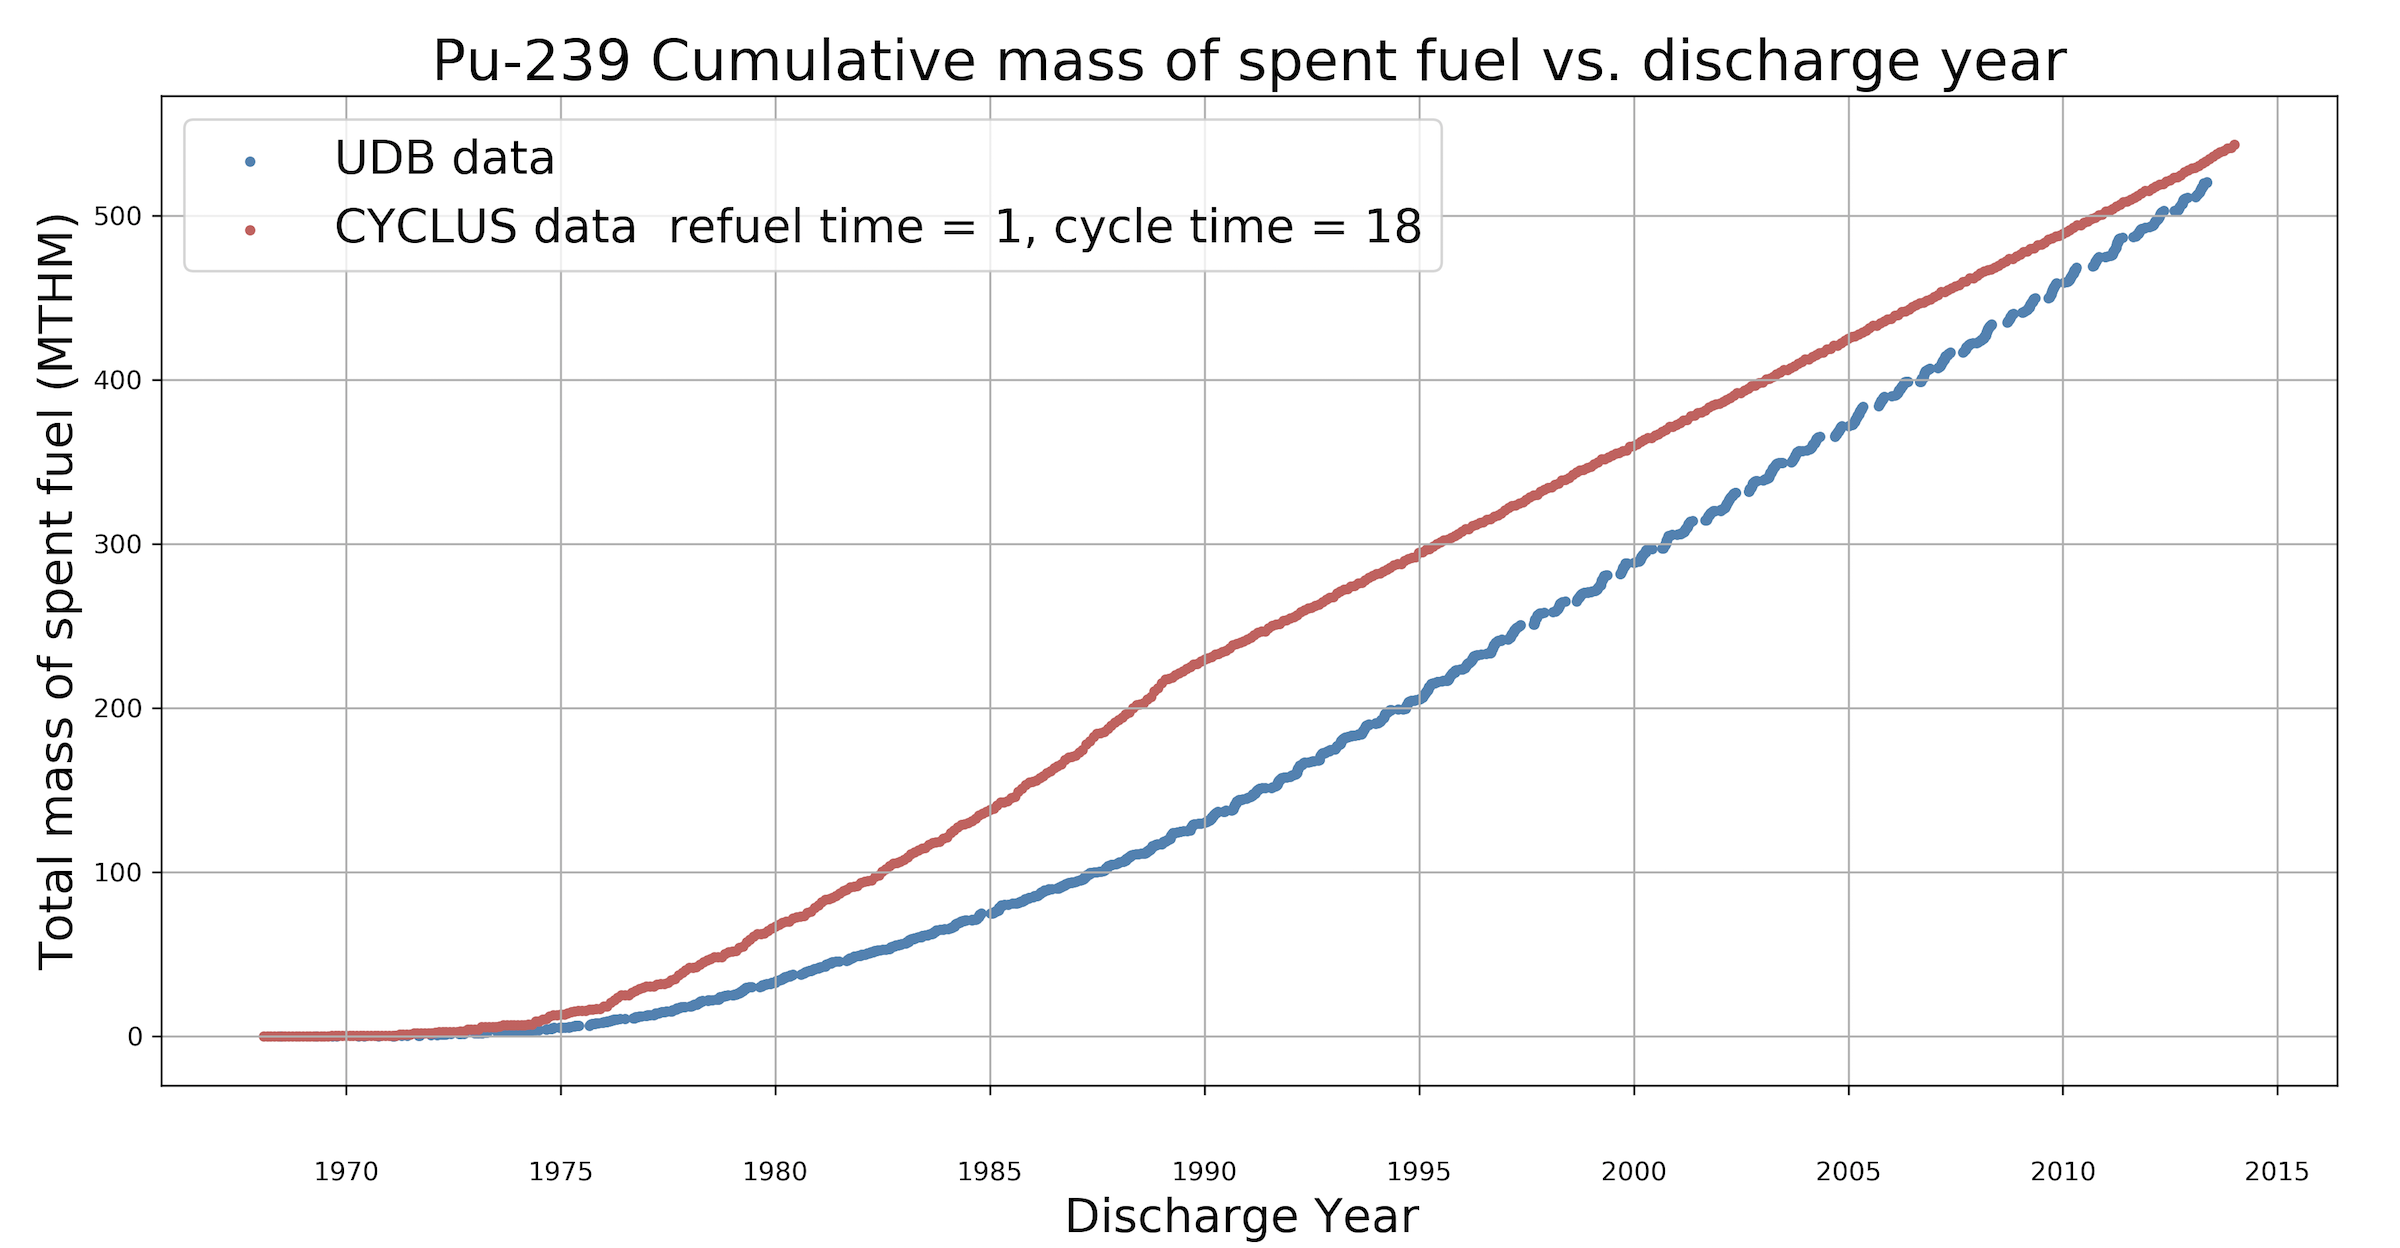
\includegraphics[width=\textwidth]{Pu-239_cumulative_mass_spent_fuel_original}
		\caption[]%
		{{\small Total cumulative Pu-239 mass in spent fuel against discharge time for \Cyclus and UDB from 1967 to 2013}}    
		\label{fig:total_pu240}
	\end{subfigure}
\caption{Total cumulative masses for specific isotopes in spent fuel against discharge time for \Cyclus and UDB from 1967 to 2013}
\end{figure}

%%%%%%%%%%%%%%%%%%%%%%%%%%%%%%%%%%%%%%%%%%%%%%%%%%%%%%%%%%%%%%%%%%%%%%%%%%%%%%%%
\section{Conclusions}
This work demonstrates that the spent fuel mass and isotopic composition results from the \Cyclus simulation of the United States nuclear fuel cycle closely follows the results from real world metrics. However, improvements can be made to replicate reality more closely. 

Further work that can improve the simulation is to give the reactor archetype, the capability to accept varying cycle and refuel times. Therefore, by looking at the historic United States reactor operating data, a \Cyclus simulation can be made to replicate their cycle and refuel times even more closely. This would give more accurate spent fuel mass and isotopic compositions which will in turn make the simulations for thermal loading of a waste repository more accurate. 

%%%%%%%%%%%%%%%%%%%%%%%%%%%%%%%%%%%%%%%%%%%%%%%%%%%%%%%%%%%%%%%%%%%%%%%%%%%%%%%%
\section{Acknowledgments}
This research is being performed using funding received from the DOE Office of Nuclear Energy's
Nuclear Energy University Program (Project 16-10512) "Demand-Driven Cycamore Archetypes". 

\pagebreak
%%%%%%%%%%%%%%%%%%%%%%%%%%%%%%%%%%%%%%%%%%%%%%%%%%%%%%%%%%%%%%%%%%%%%%%%%%%%%%%%
\bibliographystyle{ans}
\bibliography{bibliography}
\end{document}

